\section{Introduction}
	\paragraph{}{
	This chapter will outline the overall system and user interface design of the application. This will include explanations on design decisions made during the project and how the overall design will satisfy the requirements outlined in chapter 3.
	}

\section{System Design}
	\paragraph{}{
	%Intro
	The goal of the system design is to create an extensible and portable application. Any additional core features or aesthetic changes should plug in to the existing system without affecting its current functionality. This can be achieved by applying Martin Fowler's concept of the three principle layers in the design: the presentation layer, the domain layer and the data source layer.
	}
	\begin{figure}[h]
		\begin{center}
			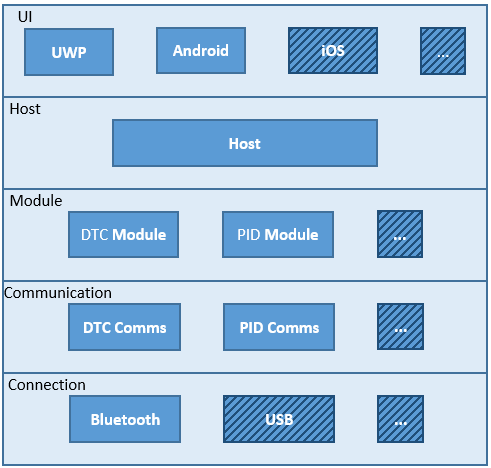
\includegraphics[width=0.8\textwidth]{Architecture.png}
			\caption{System Architecture - Only items in blue will be implemented}
		\end{center}
	\end{figure}
	\paragraph{}{
	The presentation layer represents the user interface and user input. The domain layer handles the business logic of the application, such as performing operation on data received from the data layer. The data layer represents communication with another system, such as a database or, in this case, a car. Looking at the figure 4.1, the UI layer represents the presentation layer, the connection layer represents the data layer and the host, module and communication layers can be combined to represent the domain layer.
		
	}
	\paragraph{}{
	The UI layer represents the user interface and user input handling functionality of the application. Gesture controls, such as swiping, scrolling and pinching are handled and buttons presses are hooked up to the appropriate functionality in the host or module. To port the application to another system, the developer only creates a new UI layer, as the UI is completely abstracted from the core functionality of the system.
	}
	\paragraph{}{
	The host acts as a connection between the core functionality of the application and the UI and user input. The user interface connects to the host, which grants access to the modules that are registered with it. The modules are registered with the host on initialization of the application. This means new modules can be created and added to the application, without requiring a new build.
	}
	\paragraph{}{
	The module represents the model in the MVVM pattern and a core function, such as a mode, in the system. The module contains human readable data that is retrieved from the vehicle. In order to obtain this data, the module must send a request to its communication system. The communication system, which is a part of each module, will take this request and convert it into the corresponding command that the ELM327 device and ECU can understand. It will then send this new request to the connection layer and await a response. This response, in the form of raw hexadecimal data, will be converted into a human readable value by the communication system and returned to the module, ready to be displayed or manipulated.
	}
	\paragraph{}{
	The connection layer represents the low level communication with the OBDII device, such as the ELM327 device. This layer handles the initialization and configuration of the connected device, as well as error handling, such as when the device is disconnected during a procedure or becomes out of range. All requests and responses are handled in hexadecimal format in this layer, allowing the use of raw data to be abstracted from the other layers. 
	%Initialization, Setup of device, Handles raw data
	}

\section{UI Design}
	\paragraph{}{
	It was necessary to create a coherent and highly usable user interface for this application, to satisfy the requirements of the project. This would involve creating a shared look and feel for each module in the application, so that when transitioning from one to the other, the user can easily navigate the user interface and find the functions they need to use with no learning curve.
	%Intro - Created using Pencil
	}	
	\paragraph{}{
	This was achieved by creating a UI shell, with unified controls and look and feel that would be displayed regardless of which module is currently selected. The shell acts as a means to select and view the current module as well as configure the application, such as which device is connected. Inside the shell, there is a view that the current module will occupy. Each module UI will match the color scheme, font and layout of the UI shell.
	%Microsoft UI Guideline?	
	}
	\paragraph{}{
	A number of mockups were created for the user interface using an application called Pencil. These were simple wireframes and did not include platform specific UI elements, but instead provide a more abstract view of the overall look and feel of the application. The mockups served as an initial guide when implementing the user interface and as a means of maintaining a coherent and standardised UI. 
	% UI Mockups
	}
	\paragraph{}{
		\begin{figure}[h]
			\begin{center}								
				\begin{minipage}{0.49\textwidth}
					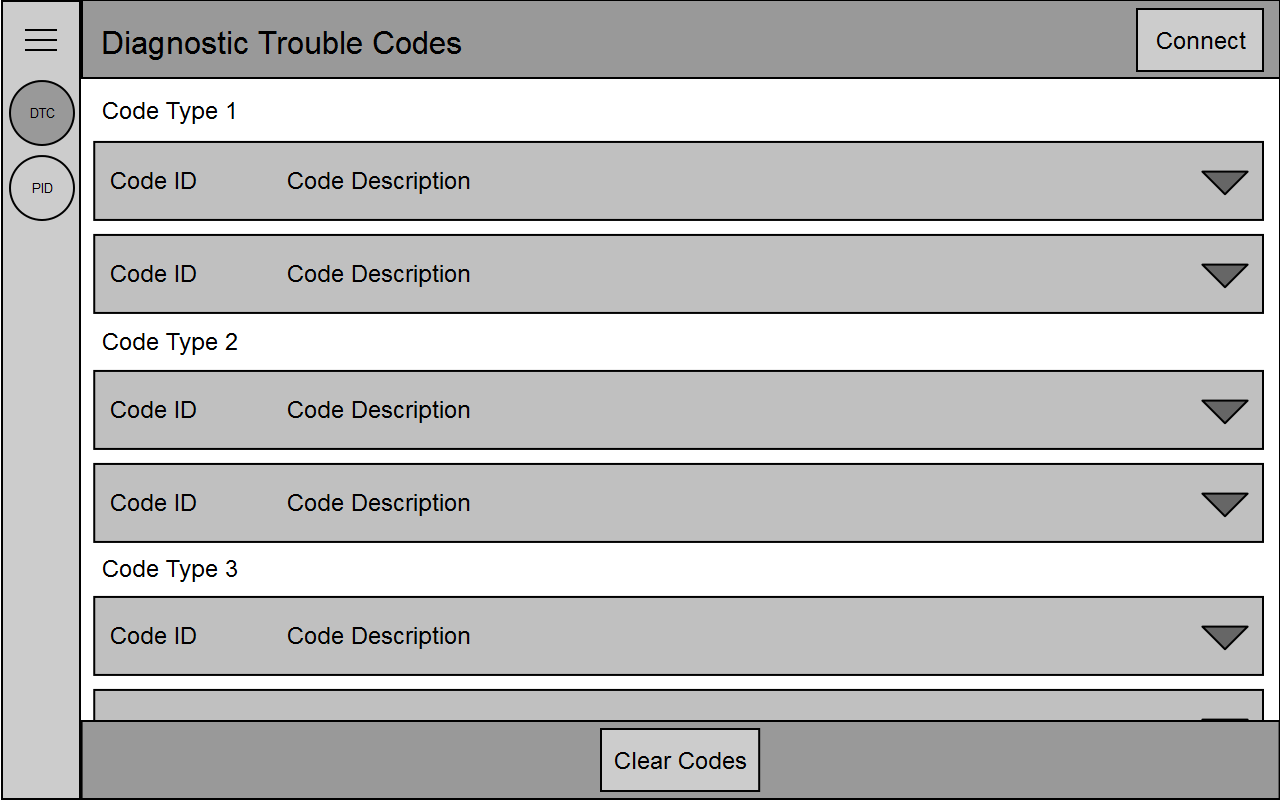
\includegraphics[width=\textwidth]{dtcpage.png}
					\caption{DTC Page}
					\vspace*{1cm}
					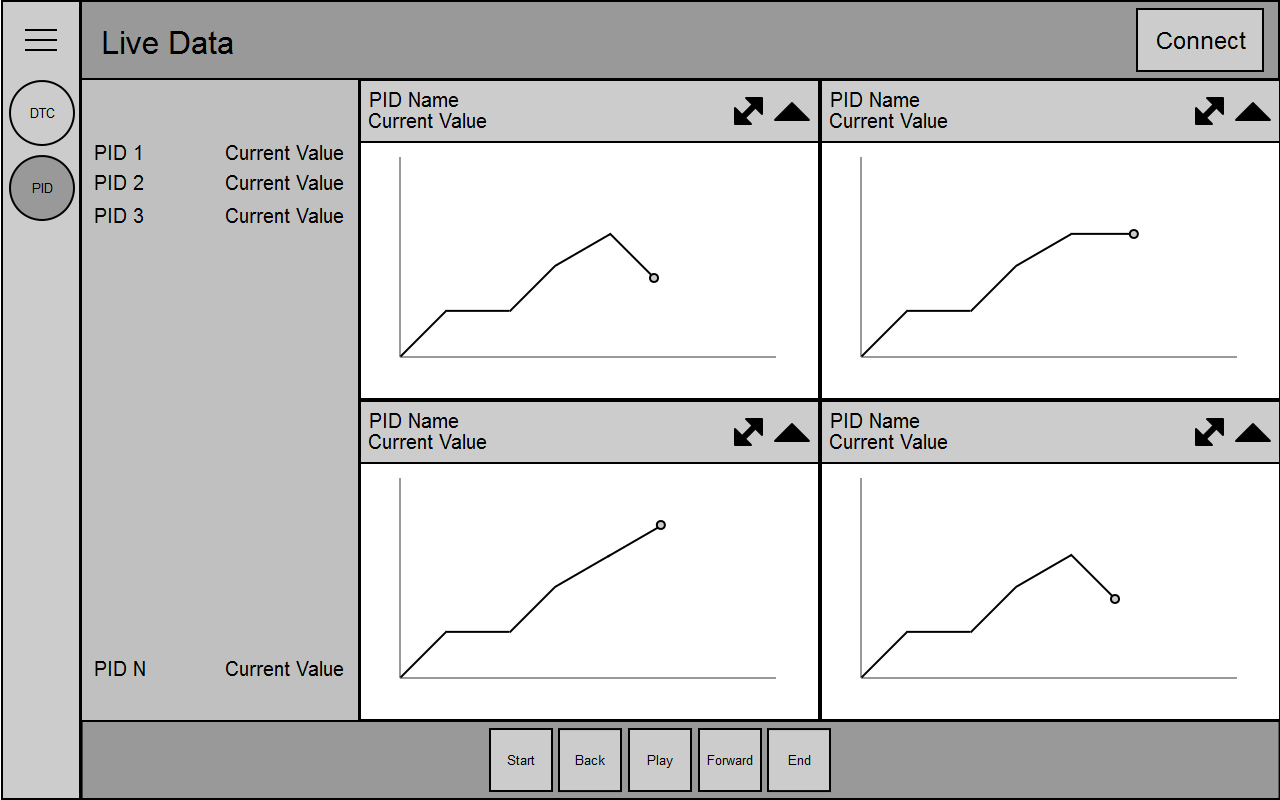
\includegraphics[width=\textwidth]{pidpage.png}
					\caption{Data Page - Graphs Expanded}						
				\end{minipage}
				\hfill			
				\begin{minipage}{0.49\textwidth}
					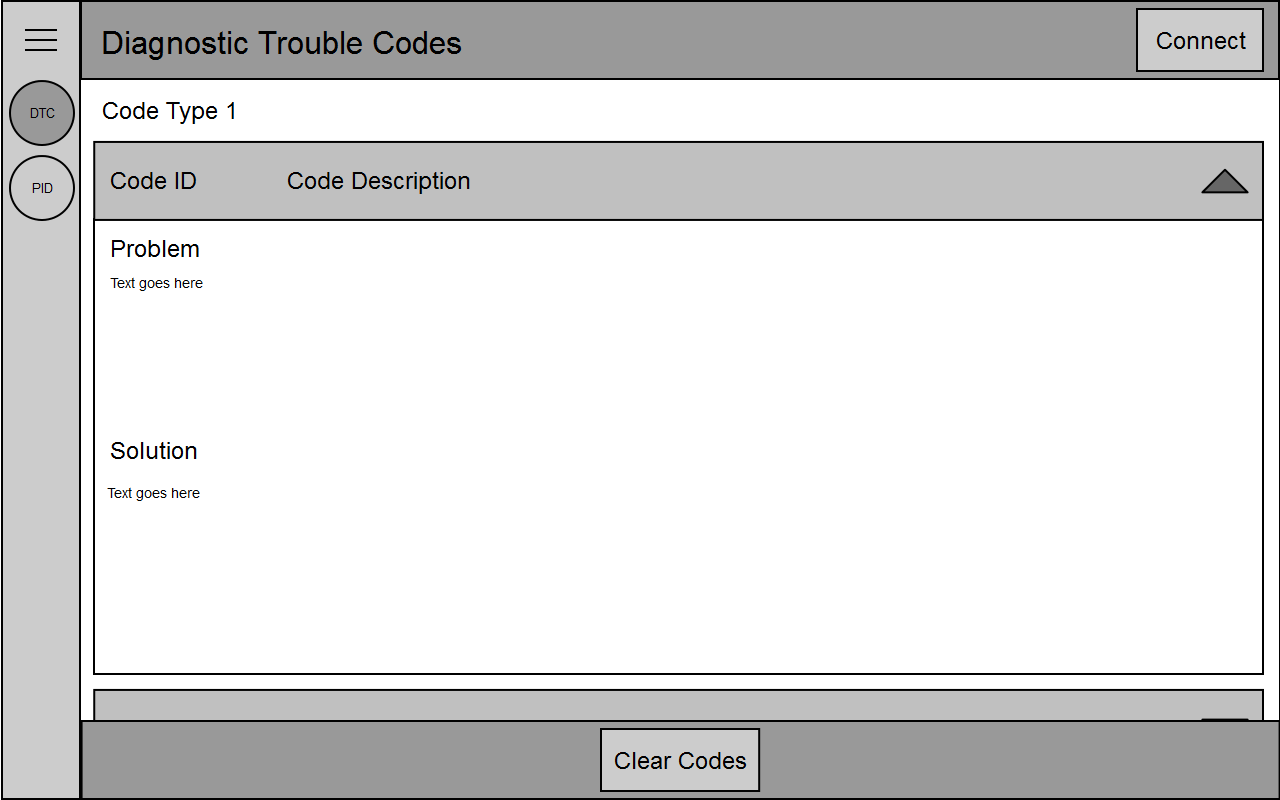
\includegraphics[width=\textwidth]{dtcpage2.png}
					\caption{DTC with information}
					\vspace*{1cm}
					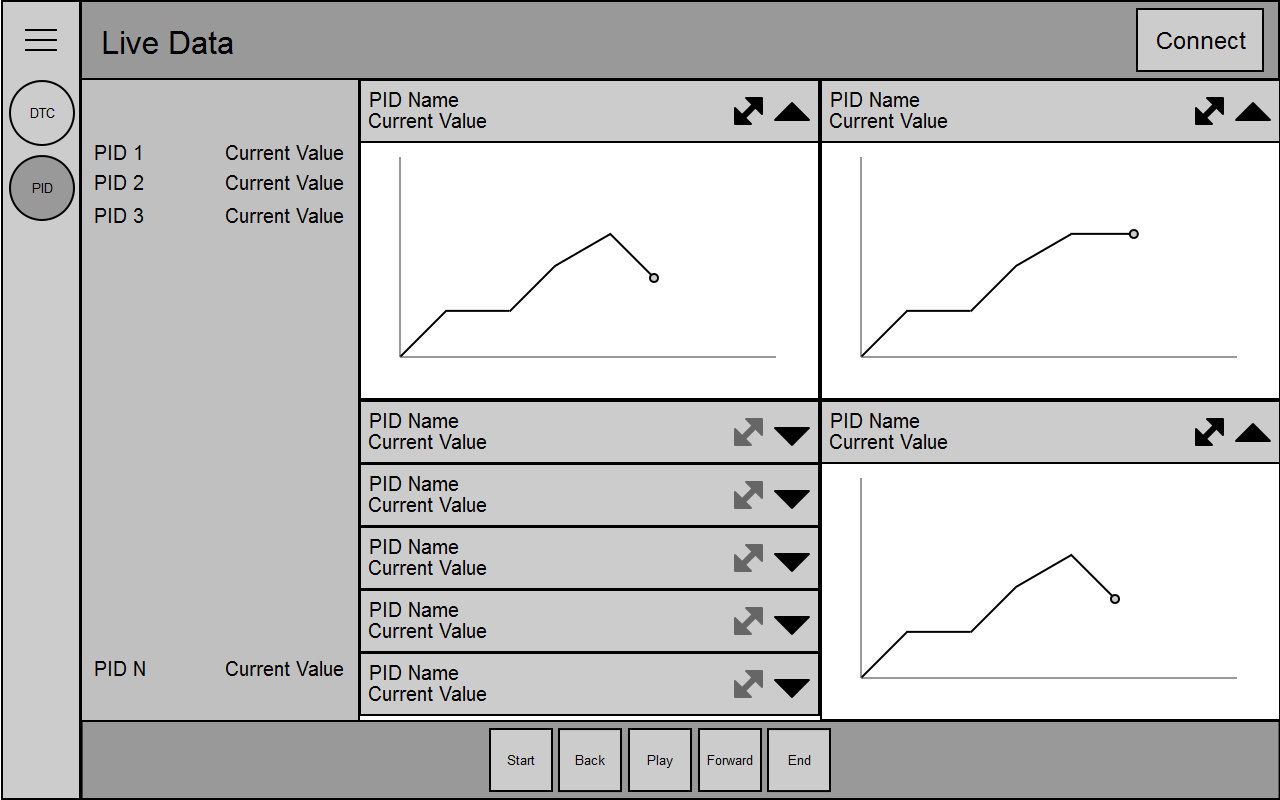
\includegraphics[width=\textwidth]{pidpage2.png}
					\caption{Data Page - Graph Collapsed}						
				\end{minipage}									
			\end{center}
		\end{figure}	
	}